\chapter{Interface générale}
La fenêtre principale de l'application est divisée en cinq parties distinctes comme le montre la figure \ref{fig:ihmClients}. 

\begin{enumerate}
	\item \textbf{Client}. Vue globale de l'ensemble des clients et des informations qui leurs sont associées	
	\item \textbf{Hiérarchie}. Actuellement composée uniquement de la liste des clients
	\item \textbf{Informations détaillées du client}. Affichage de l'ensemble des informations d’un client sélectionné
	\item \textbf{Informations détaillées de l'utilisateur}. Affichage de l'ensemble des informations de l'utilisateur sélectionné 
	\item \textbf{Recherche}. Barre de recherche et filtres associés à la recherche
	\item \textbf{Barre de menu}. Bouton d’actions raccourci
\end{enumerate}

\begin{figure}[H]
	\centering
	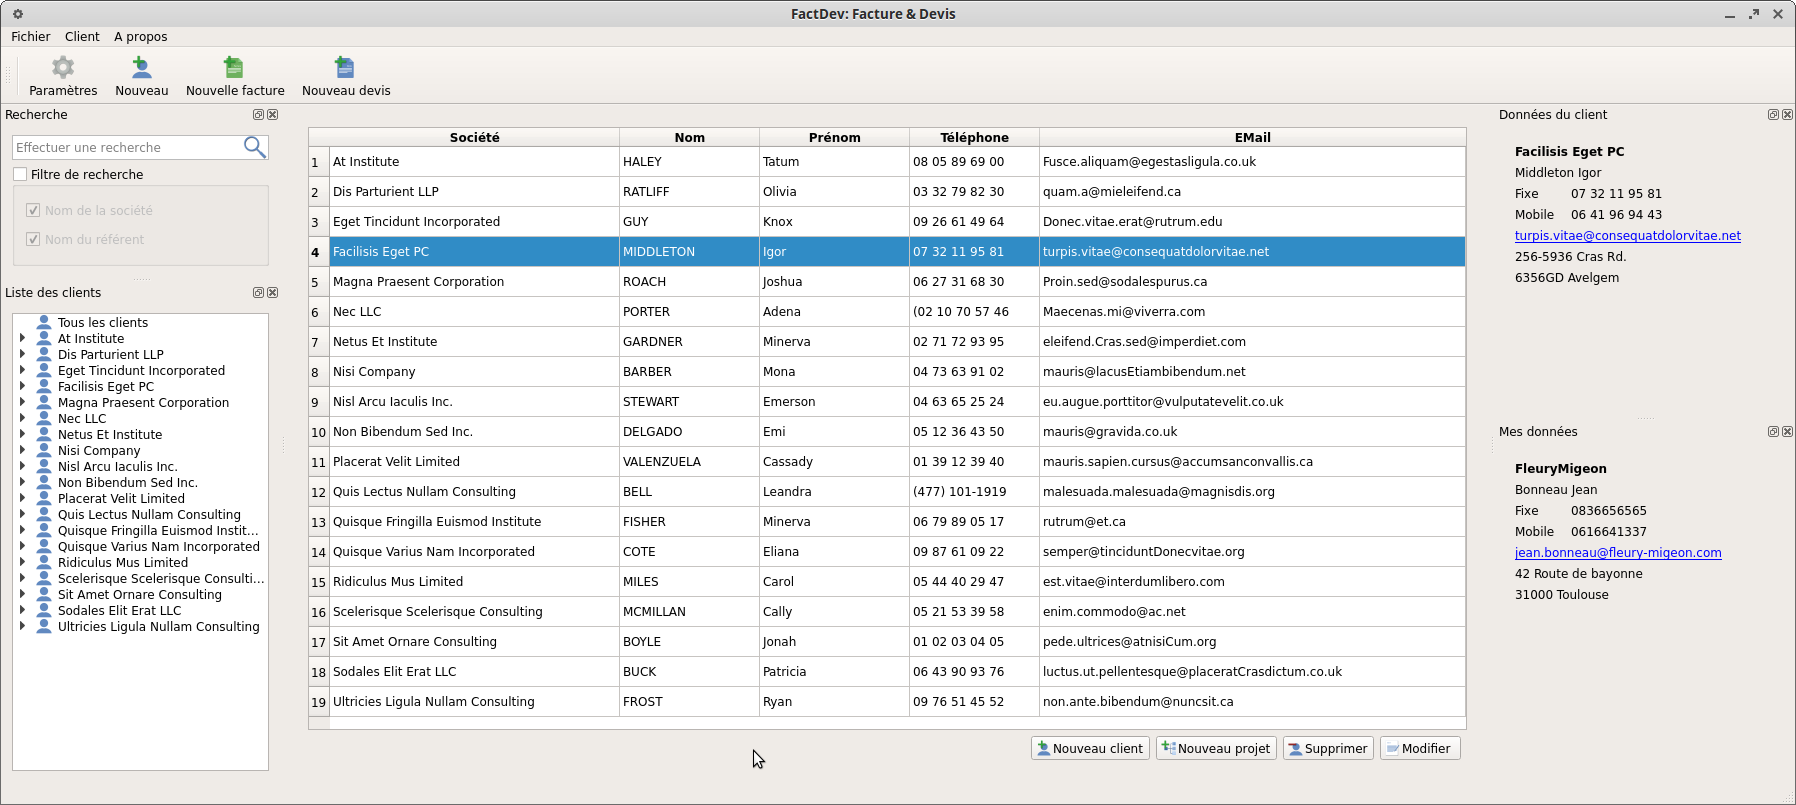
\includegraphics[width=15cm]{screens/ihmClients.png}
	\caption{Interface générale découpée en différentes parties}
	\label{fig:ihmClients}
\end{figure}

\section{Menus\index{Menus}}
La plupart des fonctionnalités du logiciel sont disponibles via les menus situés en haut de l’application. 

\subsection{Fichier\index{Menus!Fichier}}
	\begin{description}
		\item[Paramètres] Permet d'afficher\index{Utilisateur!Afficher} et d’éditer\index{Utilisateur!Éditer} l’utilisateur du logiciel.
		\item[Quitter] Quitte le logiciel
	\end{description}
\subsection{Client\index{Menus!Client}}
\begin{description}
	\item[Nouveau] Ajouter un nouveau client\index{Client!Ajouter}
	\item[Rechercher] Permet de rechercher\index{Client!Rechercher} un client dans la base de données
%	\item[Nouvelle facture]  Ajouter une nouvelle facture à un projet d’un client
%	\item[Nouveau devis] Ajouter un nouveau devis à un projet d’un client
\end{description}
\subsection{À propos\index{Menus!À propos}}
\begin{description}
	\item[Qt] Informations sur le << framework >> utilisé
	\item[Fact] Informations sur l'équipe de développement
	\item[FactDev]Informations sur le logiciel
	\item[Icons] Informations sur les icônes utilisées
\end{description}
\section{Barre d'outils\index{Barre d'outils}}
La barre d’outils permet d’effectuer certaines actions de façon rapide, actions également disponibles via le menu.

\begin{description}
	\item[Paramètres]\index{Barre d'outils!Paramètres} Permet d'afficher\index{Utilisateur!Afficher} et d’éditer l'utilisateur\index{Utilisateur!Éditer} du logiciel. Disponible via le menu <<Fichier $\rightarrow$ Paramètres>>.
	\item[Nouveau]\index{Barre d'outils!Nouveau client} Ajouter un nouveau client\index{Client!Ajouter}. Disponible via le menu <<Client $\rightarrow$ Nouveau>>.
%	\item[Nouvelle facture]  Ajouter une nouvelle facture à un projet d’un client. Disponible via le menu <<Client $\rightarrow$ Nouvelle facture>>
%	\item[Nouveau devis] Ajouter un nouveau devis à un projet d’un client. Disponible via le menu <<Client $\rightarrow$ Nouveau devis>>
\end{description}

\section{Panneau\index{Panneau} du client ou du référent\index{Panneau!Client}}
Le panneau initialement situé en haut à droite contient les informations du client\index{Client!Informations détaillées} ou du référent sélectionné, comme le montre la figure
\ref{fig:dockClient}.

\begin{figure}[H]
	\centering
	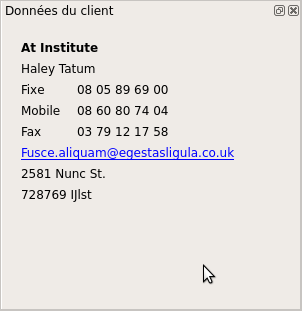
\includegraphics[height=7cm]{screens/dockClient.png}
	\caption{Panneau du client ou du référent}
	\label{fig:dockClient}
\end{figure}

\section{Panneau\index{Panneau} de l'utilisateur\index{Panneau!Utilisateur}}
Le panneau initialement situé en bas à droite contient les informations de l'utilisateur\index{Utilisateur!Informations détaillées}, comme le montre ci-dessous la figure
\ref{fig:dockUtilisateur}.

\begin{figure}[H]
	\centering
	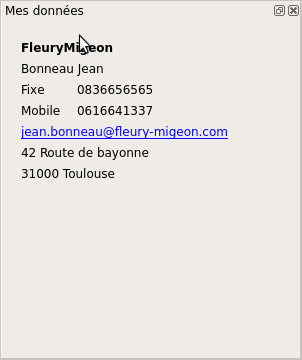
\includegraphics[height=7cm]{screens/dockUtilisateur.png}
	\caption{Panneau de l'Utilisateur}
	\label{fig:dockUtilisateur}
\end{figure}
% Il est possible d’ajouter un projet, d’en supprimer ou de modifier un projet du client via ce panneau. 
% TODO
\section{Panneau hiérarchique\index{Panneau!Hiérarchie}}
Le panneau hiérarchique, initialement situé en bas à droite de la fenêtre principale, comporte une vue hiérarchique de l'ensemble des clients et des projets associés à chacun de ces clients.

\begin{figure}[H]
	\centering
	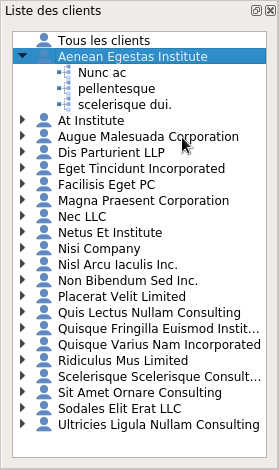
\includegraphics[width=7cm]{screens/dockHierarchique.png}
	\caption{Panneau Hiérarchique}
	\label{fig:dockHierarchique}
\end{figure}

\section{Panneau de recherche\index{Panneau!Recherche}}
Le panneau de recherche, situé en haut à la gauche, permet d’effectuer une recherche sur le nom de la société, le nom du client ou du référent si la case filtre de recherche est cochée. La recherche est alors faite selon le nom du référent. Cela permet de retrouver rapidement et facilement un client.

En dessous du champ de recherche sont affichés toutes les sociétés dans la base de données ainsi que les noms des clients ou référents lorsque ceux-ci ne possèdent pas de société.

\begin{figure}[H]
	\centering
	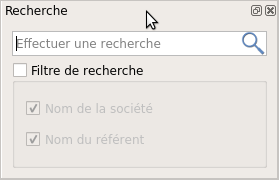
\includegraphics[width=7cm]{screens/dockRecherche.png}
	\caption{Panneau de Recherche}
	\label{fig:dockRecherche}
\end{figure}


